\begin{adjustbox}{max width=\textwidth, max totalheight=0.75\textheight, center}
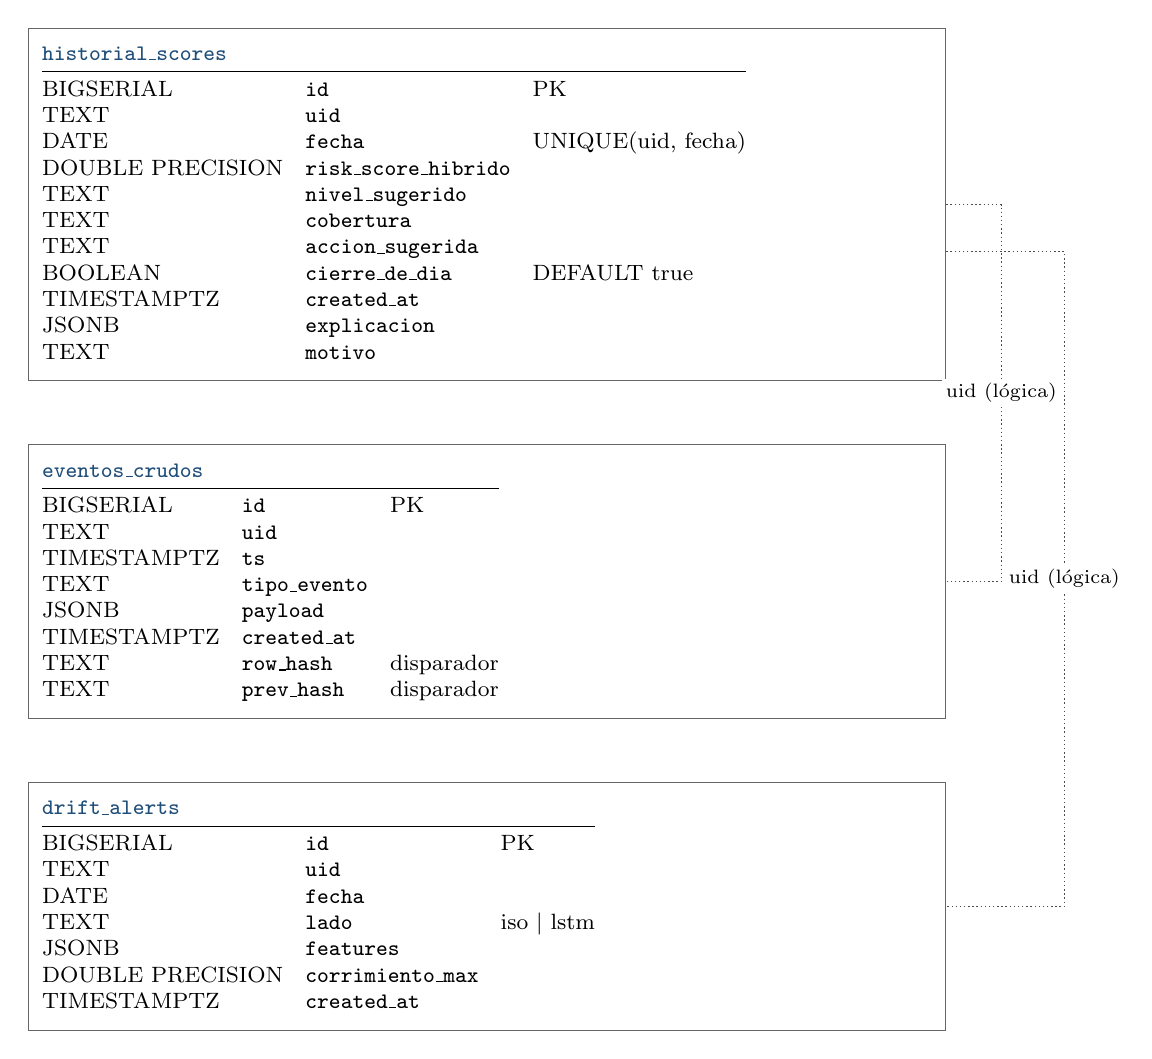
\begin{tikzpicture}[x=1cm, y=1cm]
% Estilos comunes de las figuras TikZ (despliegue y modelo relacional).
\definecolor{acento}{HTML}{1F4E79}
\hyphenpenalty=10000 \exhyphenpenalty=10000
\tikzset{
	caja/.style={draw=black!60, line width=0.4pt, fill=white, rounded corners=1pt, align=center, font=\footnotesize, inner sep=4pt, minimum height=0.9cm, text width=3.2cm},
	cajaacento/.style={caja, draw=acento, line width=0.7pt},
	opc/.style={caja, dashed, draw=black!55},
	almacen/.style={draw=black!60, line width=0.4pt, fill=black!6, cylinder, shape border rotate=90, aspect=0.22, align=center, font=\footnotesize, inner sep=3pt, minimum height=1.5cm, text width=2.6cm},
	zona/.style={draw=black!45, line width=0.4pt, fill=black!3, rounded corners=2pt, inner sep=8pt},
	zonaint/.style={draw=black!45, line width=0.4pt, fill=white, rounded corners=2pt, inner sep=7pt},
	flecha/.style={-{Stealth[length=5pt,width=4pt]}, line width=0.5pt, draw=black!70},
	rotulo/.style={font=\scriptsize, fill=white, inner sep=1.5pt},
	titulo/.style={font=\footnotesize\bfseries, text=black!75, anchor=south west},
}

\tikzset{tabla/.style={draw=black!60, line width=0.4pt, fill=white, inner sep=5pt, anchor=north west, font=\footnotesize, text width=11.3cm, align=left}}
\node[tabla] (sc) at (0,0) {%
\begin{tabular}{@{}l@{\hspace{8pt}}l@{\hspace{8pt}}l@{}}
\multicolumn{3}{@{}l@{}}{\textcolor{acento}{\textbf{\texttt{historial\_scores}}}} \\[1pt]
\hline
\noalign{\vskip 2pt}
{BIGSERIAL} & \texttt{id} & PK \\
{TEXT} & \texttt{uid} &  \\
{DATE} & \texttt{fecha} & UNIQUE(uid, fecha) \\
{DOUBLE PRECISION} & \texttt{risk\_score\_hibrido} &  \\
{TEXT} & \texttt{nivel\_sugerido} &  \\
{TEXT} & \texttt{cobertura} &  \\
{TEXT} & \texttt{accion\_sugerida} &  \\
{BOOLEAN} & \texttt{cierre\_de\_dia} & DEFAULT true \\
{TIMESTAMPTZ} & \texttt{created\_at} &  \\
{JSONB} & \texttt{explicacion} &  \\
{TEXT} & \texttt{motivo} &  \\
\end{tabular}};
\node[tabla] (ev) at ([yshift=-0.8cm]sc.south west) {%
\begin{tabular}{@{}l@{\hspace{8pt}}l@{\hspace{8pt}}l@{}}
\multicolumn{3}{@{}l@{}}{\textcolor{acento}{\textbf{\texttt{eventos\_crudos}}}} \\[1pt]
\hline
\noalign{\vskip 2pt}
{BIGSERIAL} & \texttt{id} & PK \\
{TEXT} & \texttt{uid} &  \\
{TIMESTAMPTZ} & \texttt{ts} &  \\
{TEXT} & \texttt{tipo\_evento} &  \\
{JSONB} & \texttt{payload} &  \\
{TIMESTAMPTZ} & \texttt{created\_at} &  \\
{TEXT} & \texttt{row\_hash} & disparador \\
{TEXT} & \texttt{prev\_hash} & disparador \\
\end{tabular}};
\node[tabla] (dr) at ([yshift=-0.8cm]ev.south west) {%
\begin{tabular}{@{}l@{\hspace{8pt}}l@{\hspace{8pt}}l@{}}
\multicolumn{3}{@{}l@{}}{\textcolor{acento}{\textbf{\texttt{drift\_alerts}}}} \\[1pt]
\hline
\noalign{\vskip 2pt}
{BIGSERIAL} & \texttt{id} & PK \\
{TEXT} & \texttt{uid} &  \\
{DATE} & \texttt{fecha} &  \\
{TEXT} & \texttt{lado} & iso \textbar{} lstm \\
{JSONB} & \texttt{features} &  \\
{DOUBLE PRECISION} & \texttt{corrimiento\_max} &  \\
{TIMESTAMPTZ} & \texttt{created\_at} &  \\
\end{tabular}};
\draw[densely dotted, line width=0.5pt, draw=black!70] (sc.east) -- ++(0.7,0) |- node[rotulo, pos=0.25] {uid (lógica)} (ev.east);
\draw[densely dotted, line width=0.5pt, draw=black!70] ([yshift=-0.6cm]sc.east) -- ++(1.5,0) |- node[rotulo, pos=0.25] {uid (lógica)} (dr.east);
\end{tikzpicture}
\end{adjustbox}
